\documentclass[12pt,letterpaper]{article}
\usepackage[utf8]{inputenc}
\usepackage{amsmath,amsthm,amsfonts,amssymb,amscd}
\usepackage[table]{xcolor}
\usepackage[margin=2.5cm]{geometry}
\usepackage{ragged2e}
\usepackage{graphicx}
\usepackage{multicol}
%\usepackage[brazil]{babel}
\newlength{\tabcont}
\setlength{\parindent}{0.0in}
\setlength{\parskip}{0.05in}

\begin{document}

	\large \textbf{Nome}: Luís Felipe de Melo Costa Silva \\
	\textbf{Número USP}: 9297961

	\begin{center}
		\LARGE \bf
		Lista de Exercícios 3 - MAC0425
	\end{center}

	\section*{Exercício 10.6}

	Quando os efeitos negativos de uma ação são descartados, nós adicionamos apenas os efeitos positivos, aumentando o conjunto de literais em que podemos encontrar a solução. Nesse caso, estamos simplificando as condições, tornando o problema menos restrito e mais geral, acabando com um problema mais fácil do que o original.

	\section*{Exercício 10.9}

	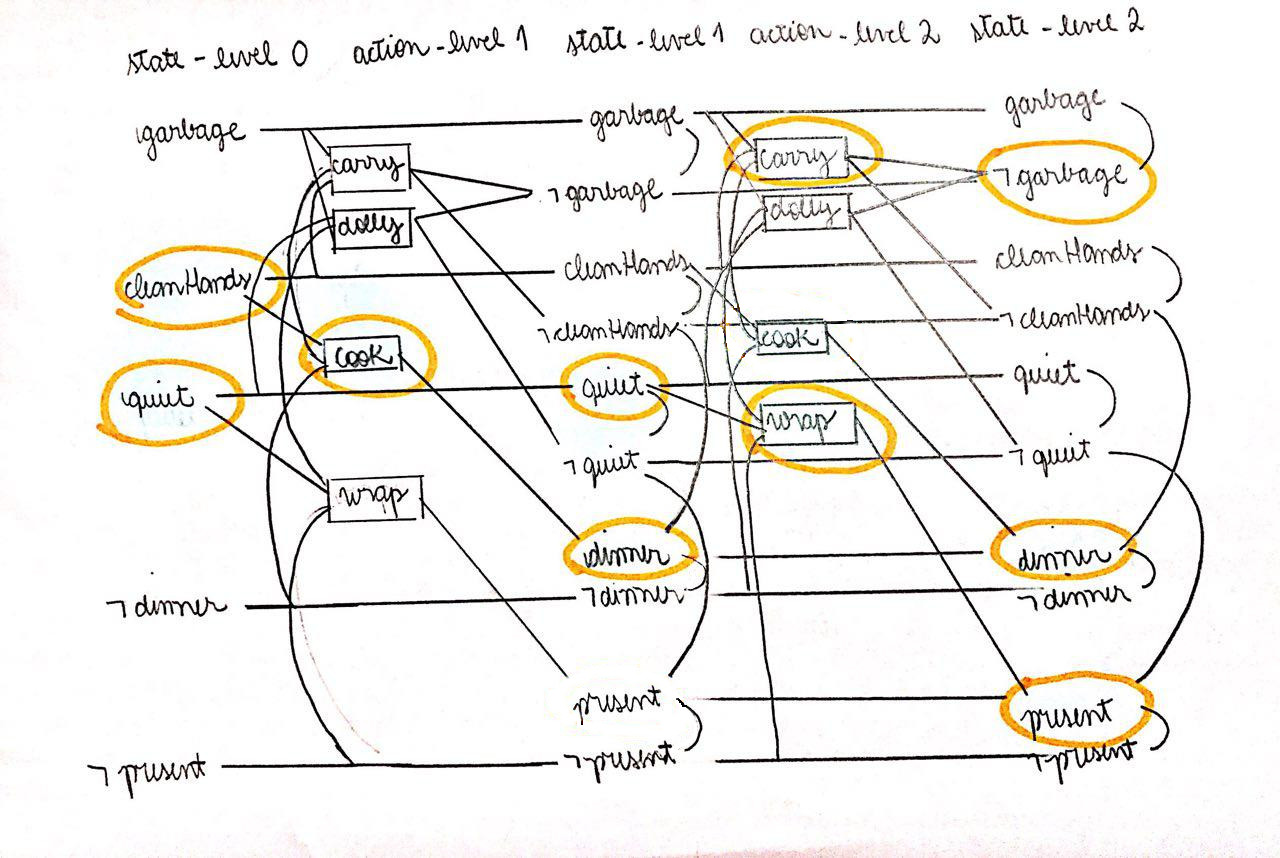
\includegraphics[width=\textwidth]{graphplan.jpg}

	\begin{itemize}
		\item Começamos o Graphplan com os sequentes literais e os que não temos da meta no \textit{state-level 0}.
		\item Então, aplicamos as ações possíveis a partir desses literais em \textit{action-level 1}. Podemos observar que:
		\begin{itemize}
			\item \textit{carry} está em mutex com \textit{cook} porque \textit{carry} elimina a pré-condição \textit{cleanHands} de \textit{cook}. (Interferência)
			\item \textit{carry} está em mutex com a manutenção para garbage. (Efeitos inconsitentes)
			\item \textit{dolly} está em mutex com \textit{wrap} porque \textit{dolly} elimina a pré-condição \textit{quiet} de \textit{wrap}. (Interferência)
		\end{itemize}
		\item Chegamos ao \textit{state-level 1}, onde todas os literais são mutex uma com a outra por suporte inconsistente (todos possuem a negação no mesmo nível). Além disso, \textit{$\lnot$quiet} está em mutex com \textit{present} e \textit{$\lnot$cleanHands} está em mutex com \textit{dinner} pelo mesmo motivo. Temos dois possíveis conjuntos de soluções: [\textit{carry, cook, wrap}] e [\textit{dolly, cook, wrap}]. Nenhuma delas é válida porque \textit{carry} está em mutex com \textit{cook} e \textit{dolly} está em mutex com \textit{wrap}. Faremos mais uma expansão do grafo.
		\item Prosseguimos para o \textit{action-level 2}, que é idêntico ao \textit{action-level 1} e gera o \textit{state-level 2}, semelhante ao \textit{state-level 1}.
	\end{itemize}

	Para encontrarmos o plano para resolver esse problema, começamos selecionando os literais da meta em \textit{state-level 2}. Então, pegamos ações no \textit{action-level 2} que não estão em mutex entre si (\textit{carry, wrap}) e as pré-condições dessas ações (\textit{quiet}) e a ação de manutenção dos literais que não foram contemplados com as ações escolhidas (\textit{dinner}), que estão no \textit{state-level 1}. Olhamos para o \textit{action-level 1} e procuramos as ações que geram \textit{dinner} e \textit{quiet}. A ação \textit{cook} gera \textit{dinner}, e \textit{quiet} é gerado por uma ação de manutenção. Logo, nosso plano é [\textit{cook, carry, wrap}]. Existem outros planos possíveis, por exemplo: [\textit{wrap, cook, dolly}].    

	\section*{Exercício MDP}

	\section*{Exercício Q-Learning}
	
	Para esse exercício vamos usar a fórmula do \textit{Q-value update}, que consiste em:
	
	\begin{center}
		$Q(s,a) \leftarrow (1-\alpha)\cdot Q(s,a) + \alpha(r+\gamma\cdot max_{a'\in A}Q(s',a'))$
	\end{center}
	
	O enunciado nos pede para usar $\alpha = 1$ e $\gamma = 0,9$. Com esses valores, nossa fórmula ficará: 
	
	\begin{center}
		$Q(s,a) \leftarrow (r+0,9\cdot max_{a'\in A}Q(s',a'))$
	\end{center}
	
	Começando com a tabela zerada e fazendo os cálculos para os episódios pedidos, teremos:
	
	\textbf{1.}
	
	$Q(3,S) = -10 + 0,9 \cdot 0 = -10$\\
	$Q(3,N) = 0 + 0,9 \cdot 0 = 0$\\
	$Q(1,N) = -10 + 0,9 \cdot 0 = -10$\\
	$Q(1,O) = 10 + 0,9 \cdot 0 = 10$\\
	
	\textbf{2.}
	
	$Q(2,L) = 0 + 0,9 \cdot 0 = 0$\\
	$Q(3,N) = 0 + 0,9 \cdot 0 = 0$\\
	$Q(1,N) = -10 + 0,9 \cdot 0 = -10$\\
	$Q(1,L) = -10 + 0,9 \cdot 0 = -10$\\	
	$Q(1,O) = 10 + 0,9 \cdot 0 = 10$\\
	
	As tabelas finais Q dos episódios calculados estão na próxima página.
	
	\newpage

	\begin{table}[]
		\centering
		\caption{Tabela do episódio da experiência 1}
		\label{my-label}
		\begin{tabular}{|l|l|l|l|l|}
			\cline{1-5}
			s/a  & \multicolumn{1}{|c|}{N}     & \multicolumn{1}{|c|}{S}       & L   & \multicolumn{1}{|c|}{O}     \\ \cline{1-5}
			0    & \multicolumn{1}{|c|}{$0$}   & \multicolumn{1}{|c|}{$0$}     & $0$ & \multicolumn{1}{|c|}{$0$}   \\ \cline{1-5}
			1    & \multicolumn{1}{|c|}{$-10$} & \multicolumn{1}{|c|}{$0$}     & $0$ & \multicolumn{1}{|c|}{$10$}  \\ \cline{1-5}
			2    & \multicolumn{1}{|c|}{$0$}   & \multicolumn{1}{|c|}{$0$}     & $0$ & \multicolumn{1}{|c|}{$0$}   \\ \cline{1-5}
			3    & \multicolumn{1}{|c|}{$0$}   & \multicolumn{1}{|c|}{$-10$}   & $0$ & \multicolumn{1}{|c|}{$0$}   \\ \cline{1-5}
		\end{tabular}
	\end{table}

	\begin{table}[]
		\centering
		\caption{Tabela do episódio da experiência 2}
		\label{my-label}
		\begin{tabular}{|l|l|l|l|l|}
			\cline{1-5}
			s/a  & \multicolumn{1}{|c|}{N}     & S       & \multicolumn{1}{|c|}{L}   & \multicolumn{1}{|c|}{O}     \\ \cline{1-5}
			0    & \multicolumn{1}{|c|}{$0$}   & $0$   & \multicolumn{1}{|c|}{$0$}   & \multicolumn{1}{|c|}{$0$}   \\ \cline{1-5}
			1    & \multicolumn{1}{|c|}{$-10$} & $0$   & \multicolumn{1}{|c|}{$-10$} & \multicolumn{1}{|c|}{$10$}  \\ \cline{1-5}
			2    & \multicolumn{1}{|c|}{$0$}   & $0$   & \multicolumn{1}{|c|}{$0$}   & \multicolumn{1}{|c|}{$0$}   \\ \cline{1-5}
			3    & \multicolumn{1}{|c|}{$0$}   & $0$   & \multicolumn{1}{|c|}{$0$}   & \multicolumn{1}{|c|}{$0$}   \\ \cline{1-5}
		\end{tabular}
	\end{table}

\end{document}
